\documentclass{article}

\usepackage{geometry}
\usepackage{amsmath}
\usepackage{graphicx}
\usepackage{listings}
\usepackage{hyperref}
\usepackage{multicol}
\usepackage{fancyhdr}
\pagestyle{fancy}
\hypersetup{ colorlinks=true, linkcolor=black, filecolor=magenta, urlcolor=cyan}
\geometry{ a4paper, total={170mm,257mm}, top=20mm, right=20mm, bottom=20mm, left=20mm}
\setlength{\parindent}{0pt}
\setlength{\parskip}{1em}
\renewcommand{\headrulewidth}{0pt}
\lhead{Competitive Programming - Arkavidia V}
\fancyfoot[CE,CO]{\thepage}
\lstset{
    basicstyle=\ttfamily\small,
    columns=fixed,
    extendedchars=true,
    breaklines=true,
    tabsize=2,
    prebreak=\raisebox{0ex}[0ex][0ex]{\ensuremath{\hookleftarrow}},
    frame=none,
    showtabs=false,
    showspaces=false,
    showstringspaces=false,
    prebreak={},
    keywordstyle=\color[rgb]{0.627,0.126,0.941},
    commentstyle=\color[rgb]{0.133,0.545,0.133},
    stringstyle=\color[rgb]{01,0,0},
    captionpos=t,
    escapeinside={(\%}{\%)}
}

\begin{document}

\begin{center}
    \section*{C. Cincin Arvy}

    \begin{tabular}{ | c c | }
        \hline
        Batas Waktu  & 1s \\
        Batas Memori & 512MB \\
        \hline
    \end{tabular}
\end{center}

\subsection*{Deskripsi}

Arvy yang sudah beranjak dewasa pergi kesebuah toko perhiasan. Disana Arvy membeli sebuah cincin untuk hadiah kekasih barunya.
Namun Arvy yang kurang beruntung pada hari itu.
Sesaat Arvy keluar dari toko, cincin arvy dirampas oleh seorang penjahat.
Kemudian penjahat tersebut berlari melewati rel kereta yang lebarnya $d$ meter.

Arvy ingin melewati rel kereta tersebut, namun tepat sebuah kereta akan melintas dengan kelajuan $v_k$ meter per sekon.
Saat ini Arvy sedang berada $y$ meter dari rel dan dapat berlari dengan kecepatan $v_a$ meter per sekon.
Kepala kereta berjarak $\sqrt{x^2+y^2}$ meter dari Arvy.
Posisi Arvy, kereta, dan rel dapat digambarkan seperti berikut:

\begin{center}
    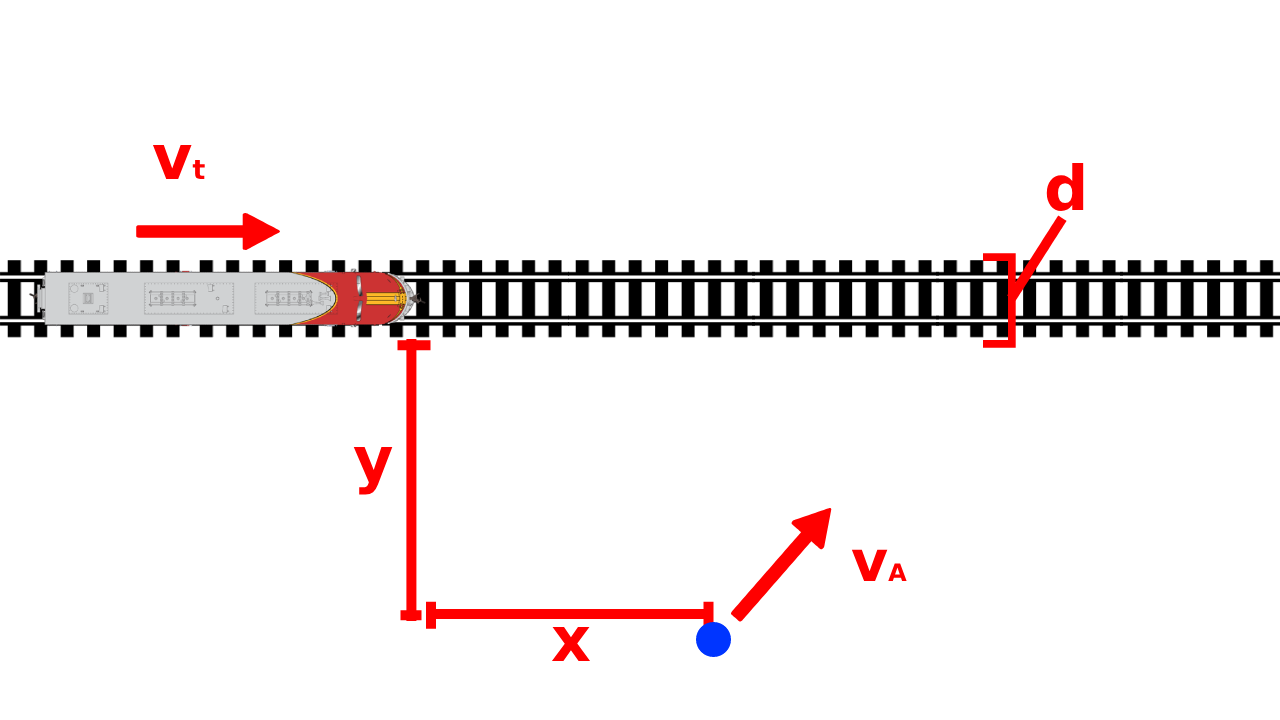
\includegraphics[width=200px]{skema}
\end{center}

Arvy dapat berlari lurus, bergerak parabola, atau berputar-putar, namun tidak melebih kecepatan $v_a$ meter per sekon.
Apakah Arvy dapat mendahului kereta untuk melalui rel kereta tersebut dan mendapatkan kembali cincin yang ingin Arvy hadiahkan untuk kekasihnya?

\subsection*{Format Masukan}
Baris pertama terdiri dari satu bilangan bulat positif $T$ ($1 \leq T \leq 1.000$), menyatakan banyaknya kasus uji.
Tiap kasus uji terdiri dari bilangan $d, x, y, v_k, v_a$ ($1 \leq d, x, y, v_k, v_a \leq 1.000.000.000$) menyatakan lebar rel kereta, jarak horizontal Arvy dengan kereta, jarak vertikal Arvy dengan kereta, kecepatan kereta, dan kecepatan Arvy.

\subsection*{Format Keluaran}
Untuk tiap kasus uji, keluarkan \lstinline{YA} jika Arvy dapat menyebrangi rel, atau \lstinline{TIDAK} jika tidak.

\begin{multicols}{2}
\subsection*{Contoh Masukan}
\begin{lstlisting}
3
1 100 1 5 20
1 10 20 10 5
1 4 6 5 5
\end{lstlisting}
\columnbreak
\subsection*{Contoh Keluaran}
\begin{lstlisting}
YA
TIDAK
YA
\end{lstlisting}
\vfill
\null
\end{multicols}

\end{document}